%%%%%%%%%%%%%%%%%%%%%%%%%%%%%%%%%%%%%%%%%%%%%%%%%%%%%%%%%%%%%%%%%%%%%%%%%%%
%
% Generic template for TFC/TFM/TFG/Tesis
%
% $Id: estudioTeorico.tex,v 1.5 2015/06/05 00:05:19 macias Exp $
%
% By:
%  + Javier Macías-Guarasa.
%    Departamento de Electrónica
%    Universidad de Alcalá
%  + Roberto Barra-Chicote.
%    Departamento de Ingeniería Electrónica
%    Universidad Politécnica de Madrid
% 
% Based on original sources by Roberto Barra, Manuel Ocaña, Jesús Nuevo, Pedro Revenga, Fernando Herránz and Noelia Hernández. Thanks a lot to all of them, and to the many anonymous contributors found (thanks to google) that provided help in setting all this up.
%
% See also the additionalContributors.txt file to check the name of additional contributors to this work.
%
% If you think you can add pieces of relevant/useful examples, improvements, please contact us at (macias@depeca.uah.es)
%
% You can freely use this template and please contribute with comments or suggestions!!!
%
%%%%%%%%%%%%%%%%%%%%%%%%%%%%%%%%%%%%%%%%%%%%%%%%%%%%%%%%%%%%%%%%%%%%%%%%%%%

\chapter{Estado del arte}\label{cha:estado-arte}

En este capítulo, se lleva a cabo la explicación de distintos aspectos teóricos esenciales para el entendimiento del desarrollo del proyecto.
Para ello, este capítulo se dividirá en cinco apartados.

\section{Criptografía}\label{sec:criptografia}


\subsection{Características}\label{subsec:caracteristicas}


\subsection{Modelos actuales}\label{subsec:mod_act}


\subsection{Computación cuántica}\label{subsec:cuantica}


\subsection{Criptografía postcuántica}\label{subsec:postcuantica}

\subsubsection{Dilithium}\label{subsubsec:dilithium}

Dilithium~\cite{dilithium} es un algoritmo criptográfico de firma digital basado en retículos.
Este algoritmo fue seleccionado por el \ac{NIST} como estándar para un sistema de firma postcuántica~\cite{nist_sel}.

El esquema Dilithium se basa en Fiat-Shamir con abortos~\cite{10.1007/978-3-642-10366-7_35} y consta de tres funciones principales: una función de generación de claves, una función de firma y una función de comprobación de firma~\cite{dilithium_spec}.
En cuanto a la generación de las claves, se proporciona el Algoritmo~\ref{alg:gen_dilithium}.
En este proceso, se genera una matriz A de dimensiones $k \times l$ y, posteriormente, se obtienen vectores aleatorios de la clave secreta.

\begin{algorithm}
    \caption{Generación de claves pública y privadas en Dilithium~\cite{dilithium_spec}.}
    \label{alg:gen_dilithium}
    %\KwData{Nada}
    \KwResult{Claves pública y privada.}
    \hspace{2mm}$\textbf{A} \gets R_q^{k\times l}$\newline
    $(s_1,s_2) \gets S_\eta^l \times S_\eta^{k}$\newline
    $\textbf{t} := \textbf{A}s_1 + s_2$\newline
    \textbf{return} (pk = (\textbf{A}, \textbf{t}), sk = (\textbf{A}, \textbf{t}, $s_1$, $s_2$))
\end{algorithm}

En lo respectivo a la firma, esta se muestra en el algoritmo~\ref{alg:sign_dilithium}.
En él, se genera un vector de enmascaramiento de polinomios \textbf{y} con coeficientes menores que $\gamma_1$.
El parámetro $\gamma_1$ se escoge de forma que sea lo suficientemente grande como para no revelar la clave secreta pero no demasiado grande como para que la firma sea fácilmente falsificable.
A continuación, establece $w_1$ como los bits de mayor orden del cómputo \textbf{Ay} y obtiene c como la función resumen del mensaje y $w_1$.
Para evitar que \textbf{z} filtre la clave privada, se lleva a cabo una comprobación de que los componentes de \textbf{z} son menores que $\gamma_1 - \beta$.
En caso contrario, se reinicia el procedimiento.

\begin{algorithm}
    \caption{Firma en Dilithium~\cite{dilithium_spec}.}
    \label{alg:sign_dilithium}
    \KwData{Clave privada y mensaje a firmar.}
    \KwResult{Firma digital.}
    \hspace{2mm}$\textbf{z} := \perp$\newline
    \While{$z = \perp$}{
        \hspace{2mm}$y \gets S_{\gamma 1-1}^l$\newline
        $w_1 := HighBits(\textbf{Ay}, 2\gamma_2)$\newline
        $c\in B_\tau := H(M||w_1)$\newline
        $\textbf{z} := \textbf{y} + cs_1$\newline
        \If{$||z||_{\infty}\geq \gamma_1-\beta$ or $||LowBits(\textbf{Ay} - cs_2, 2\gamma_2)||_\infty\geq \gamma_2 - \beta$}{
            $\textbf{z} := \perp$
        }
    }
    \textbf{return} $\sigma = (\textbf{z}, c)$
\end{algorithm}

Finalmente, para el sistema de verificación de firma, se dispone del algoritmo~\ref{alg:ver_dilithium}.
En esta función, se computa ${w'}_1$ como los bits de mayor orden de \textbf{Az}-ct y acepta si todos los coeficientes de \textbf{z} menores que $\gamma_1 - \beta$ y si c es el resultado de la función resumen del mensaje y ${w'}_1$.

\begin{algorithm}
    \caption{Verificación de firma en Dilithium~\cite{dilithium_spec}.}
    \label{alg:ver_dilithium}
    \KwData{Clave pública y mensaje firmado.}
    \KwResult{Mensaje original.}
    \hspace{2mm}${w'}_1 := HighBits(\textbf{Ay}, 2\gamma_2)$\newline
    \If{$[||\textbf{z}||_\infty < \gamma_1 - \beta]$ \textbf{and} $[c = H(M||{w'}_1)]$}{
        \textbf{return}
    }
\end{algorithm}

Los algoritmos~\ref{alg:gen_dilithium},~\ref{alg:sign_dilithium} y~\ref{alg:ver_dilithium} son la versión simplificada pero menos eficiente del algoritmo.
Se ha decidido explicar brevemente estos diseños para otorgar un conocimiento aceptable pero no total ya que, con el entendimiento de dichos algoritmos, es suficiente.

Dilithium consta de tres versiones: Dilithium2, Dilithium3 y Dilithium5.
La diferencia entre estas consiste en el tamaño de las claves y firmas generadas.
En la tabla~\ref{tab:dilithium} se muestran los distintos tamaos a tener en cuenta de cada versión del algoritmo.
Además, se indica la seguridad ante el ataque Quantum Core-SVP tanto con \ac{SIS} como con \ac{LWE}.

\begin{table}[H]
    \centering
    \begin{tabular}{|c|c|c|c|}
    \hline
                            & \textbf{Dilithium2}   & \textbf{Dilithium3}   & \textbf{Dilithium5}   \\ \hline
    Clave pública (bytes)   & 1312                  & 1952                  & 2592                  \\ \hline
    Clave privada (bytes)   & 2528                  & 4000                  & 4864                  \\ \hline
    Firma (bytes)           & 2420                  & 3293                  & 4595                  \\ \hline
    Seguridad ante LWE (bits) & 112                 & 165                   & 229                   \\ \hline
    Seguridad ante SIS (bits) & 112                 & 169                   & 241                   \\ \hline
    \end{tabular}
    \caption{Diferencias entre versiones de Dilithium.}
    \label{tab:dilithium}
\end{table}



\subsubsection{Kyber}\label{subsubsec:kyber}


\begin{algorithm}
    \caption{Generación de claves en Kyber~\cite{kyber_spec}.}
    \label{alg:gen_kyber}
    %\KwData{}
    \KwResult{Claves pública y privada.}
    \hspace{2mm}$d \gets B^{32}$\newline
    $\rho\sigma := G(d)$\newline
    $N := 0$\newline
    \For{i from 0 to k-1}{
        \For{j from 0 to k-1}{
            Â$[i][j] := Parse(XOF(\rho, j, i))$
        }
    }
    \For{i from 0 to k-1}{
        $s[i] := CBD_{\eta 1}(PRF(\sigma, N))$\newline
        N := N + 1
    }
    \For{i from 0 to k-1}{
        $e[i] := CBD_{\eta 1}(PRF(\sigma, N))$\newline
        N := N + 1
    }
    %$a$\newline
\end{algorithm}


\subsubsection{Sphincs}\label{subsubsec:sphincs}

\subsubsection{McEliece}\label{subsubsec:mceliece}

\subsubsection{HQC}\label{subsubsec:hqc}

\subsubsection{Falcon}\label{subsubsec:falcon}




\section{IoT}\label{sec:iot}

Una vez comentados los algoritmos empleados a lo largo de este proyecto, se continúa explicando los distintos dispositivos con los que se ha llevado a cabo este trabajo.

\subsection{ESP32}\label{subsec:esp32}

El primero de estos dispositivos es el \ac{SoC} ESP32, desarrollado por Espressif Systems.
Más concretamente, se utilizará la versión ESP32-WROOM-32E~\cite{esp32-spec}.
En la Figura~\ref{fig:esp32-pinout}, se muestra el sistema Devkitc v4 que hace uso del dispositivo ESP32 anteriormente mencionado.

\begin{figure}[h]
    \centering
    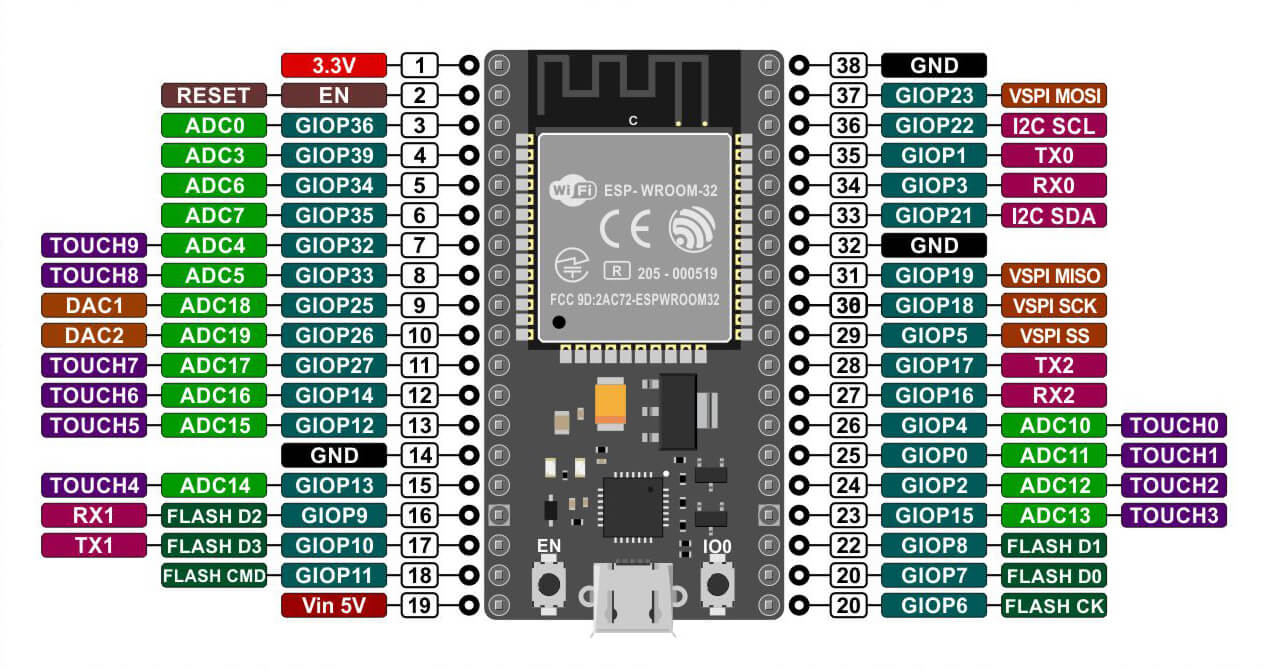
\includegraphics[width=0.8\textwidth]{figures/esp32-pinout.jpg}
    \caption{ESP32-WROOM-32E en Devkitc v4 con \textit{pinout}~\cite{esp32-pinout}.}
    \label{fig:esp32-pinout}
\end{figure}

Esta versión del \ac{SoC} dispone de un microprocesador de 32-bit Xtensa LX6 con 2 núcleos a una frecuencia máxxima de 240 MHz.
En cuanto a memoria, incluye 520 kB de memoria SRAM, 448 kB de memoria ROM y 4, 8 o 16 MB de memoria \textit{flash}.

Respecto a las comunicaciones, este dispositivo puede hacer uso del estándar 802.11 b/g/n al igual que Bluetooth v4.2 y Bluetooth LE.
Para estos estándares, incluye una antena en la parte superior, como se puede apreciar en la Figura~\ref{fig:esp32-pinout}.

Por otro lado, este dispositivo incluye una serie de periféricos como \ac{SPI}, \ac{UART}, \ac{SDIO}, \ac{I2C} y \ac{GPIO}.



\subsection{RP2040}\label{subsec:RP2040}

Por otro lado, disponemos del microcontrolador RP2040~\cite{rp2040-spec}.
Este microcontrolador se puede apreciar en varios dispositivos como Raspberry Pi Pico y Raspberry Pi Pico W.
La primera de ellas se puede apreciar en la Figura~\ref{fig:raspberry-pico}.

\begin{figure}[h]
    \centering
    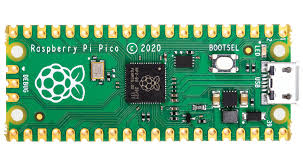
\includegraphics[width=0.6\textwidth]{figures/raspberry-pico.jpeg}
    \caption{Raspberry Pi Pico~\cite{rp2040-img}.}
    \label{fig:raspberry-pico}
\end{figure}

Este microcontrolador consta de dos procesadores ARM Cortex-M0+ a una frecuencia de 133 MHz.

En cuanto a memoria, dispone de 264 kB de SRAM en seis bancos independientes y soporta el uso de una memoria \textit{flash} de 16 MB a través de un bus QSPI.
Además, cuenta con un controlador \ac{DMA}.

En cuanto a comunicaciones, este dispositivo cuenta 2 módulos \ac{UART}, 2 controladores \ac{SPI} y 2 controladores \ac{I2C}.

En lo que respecta a periféricos, este microcontrolador dispone de 30 pines \ac{GPIO}, de los cuales 4 pueden ser utilizados como entradas analógicas.


\subsection{STM32}\label{subsec:stm32}

Por último, tenemos la familia de dispositivos STM32 basados en los procesadores ARM Cortex-M.
Esta familia está compuesta por un gran número de dispositivos.
De todos ellos, se va a proceder a explicar las características de STM32L4R5ZIT6U~\cite{nucleo-spec}.
Esto se debe a que se utilizará el dispositivo NUCLEO-L4R5ZI, el cual hace uso de microcontrolador STM32L4R5ZIT6U.
En la Figura~\ref{fig:nucleo-l4r5zi} se puede apreciar el dispositivo NUCLEO-L4R5ZI.

\begin{figure}[h]
    \centering
    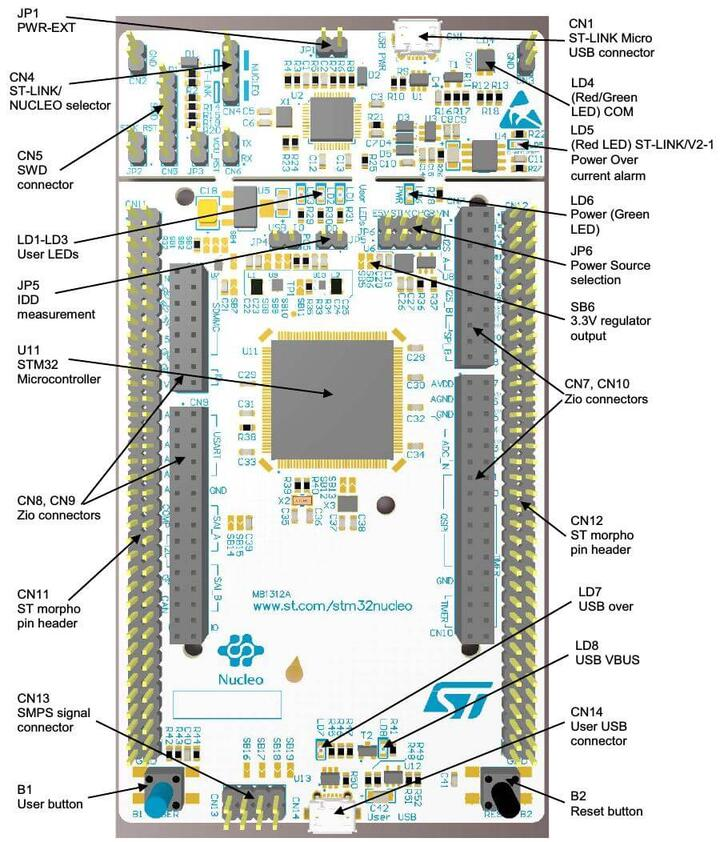
\includegraphics[width=0.6\textwidth]{figures/nucleo-l4r5zi.jpg}
    \caption{Diagrama del dispositivo NUCLEO-L4R5ZI~\cite{nucleo-img}.}
    \label{fig:nucleo-l4r5zi}
\end{figure}

El microcontrolador STM32L4R5ZIT6U consta de un procesador Arm Cortex-M4 de 32 bits con una frecuencia de hasta 120 MHz.

En lo referente a la memoria, este dispositivo dispone de una memoria \textit{flash} de 2 MB, 640 kB de memoria SRAM y una interfaz para memoria externa.
Además, dispone de un controlador \ac{DMA} con 14 canales.

Respecto a las comunicaciones, este dispositivo contiene una interfaz \ac{USB}, dos interfaces \ac{SAI}, cuatro interfaces \ac{I2C}, seis interfaces \ac{USART}, tres interfaces \ac{SPI} y un bus \ac{CAN}.



%%% Local Variables:
%%% TeX-master: "../book"
%%% End:
